\chapter{Werkzeuggestützte Analyse}


\section{Lernziele}

\begin{itemize}
    \item grundlegende Arten von qualitätssichernden Maßnahmen kennen
    \item grundlegende Arten von qualitätssichernden Maßnahmen nach verschiedenen Gesichtspunkten kategorisieren können
\end{itemize}

\newpage

\section{Einleitung}

Manuelle Verfahren sind ein effektives Mittel zur Suche nach Defekten.\\
Ihr Nachteil ist, dass ihre Durchführung sehr aufwändig ist.\\
Außerdem stellen manche Prüfarten für Menschen eher eintönige und fehleranfällige Tätigkeiten dar.\\

\noindent
Verschiedene Arten von Analysen können mit extra dafür entwickelten Werkzeugen automatisiert erfolgen, und lassen sich damit damit effizienter und zuverlässiger erledigen (vgl.~\cite[27]{Wed09c})

\noindent
Mit Hilfe der \textbf{werkzeuggestützten Analyse} kann u.a

\begin{itemize}
    \item die \textbf{Einhaltung von Programmierrichtlinien} überprüft werden
    \item nach \textbf{verdächtigen Mustern} im Code gesucht werden
    \item Defekte im Code aufspüren, die durch Fehlersituationen in Programmabläufen entstehen
\end{itemize}

\section{Programmierrichtlinien}\label{sec:programmierrichtlinien}

\subsection*{Einhaltung der Programmierrichtlinien wichtig für Wartbarkeit}

Die \textbf{Einhaltung von Programmierrichtlinien} ist eine naheliegende Aufgabe für die \textbf{werkzeuggestützte Analyse}.\\
\textbf{Programmierrichtlinien} können \textbf{projektweit}, \textbf{unternehmensweit} oder \textbf{weltweit} (wie bei Java\footnote{
s. \url{https://www.oracle.com/java/technologies/javase/codeconventions-introduction.html}, abgerufen 24.05.2024
}) vorgegeben sein.\\

\begin{tcolorbox}[colback=white]
Die Einhaltung von Programmierrichtlinien ist wichtig für die \textbf{Qualitätsforderung} \textbf{Wartbarkeit}: \textbf{Wartbarkeit} setzt auch voraus, dass der Code verständlich und damit einfach lesbar ist.
\end{tcolorbox}
\vspace{2mm}

\subsection*{Ursachen für gefundene Defekte}
Ein erster Einsatz solcher Werkzeuge ist meist sehr ernüchternd: Oft werden mehr Defekte angezeigt, als praktischerweise behoben werden können.
Die hängt u.a. damit zusammen, dass

\begin{enumerate}
    \item die Einstellungen der IDE meistens nicht mit der Einstellung der Analysewerkzeuge zusammenpassen
    \item viele Entwickler die Programmierrichtlinien nicht gut genug kennen
    \item manche der standardmäßig vorgegebenen Programmierrichtlinien für die Praxis zu strikt sind
\end{enumerate}

\noindent
Bei existierendem Code sind \textit{nachträgliche} Programmierrichtlinien schwer durchzusetzen.
Es ist denkbar, in solchen Fällen die Programmierrichtlinien nur für \textit{neuen} Code durchzusetzen.

\subsection*{Vorgehen}
\begin{itemize}
    \item Werkzeuge sollten von Anfang an benutzt werden, da ein nachträglicher Einsatz mit hohem Aufwand verbunden ist
    \item die Einführung sollte zunächst an einem kleinen Stück Software erprobt werden, die Einstellungen der IDE werden dann anhand des Beispiels angepasst, Regeln ggf. modifiziert
    \item während des ersten Gebrauchs sollten die Regeln systematisch auf die Brauchbarkeit überprüft und Werkzeug und IDE  angepasst werden, bis ein akzeptabler Stand erreicht ist
    \item die Projektleitung sollte darauf achten, dass alle Entwickler den Quellcode gleich prüfen - das Werkzeug sollte also in die IDE integriert sein, zumindest aber in das Build-Management, damit die Prüfung automatisch und periodisch durchgeführt wird
\end{itemize}

\subsection*{Werkzeuge}
Für Java gibt es für die Einhaltung von Programmierrichtlinien bspw. \textit{Checkstyle}\footnote{
    \url{https://checkstyle.org}, abgerufen 24.05.2024
}, für JavaScript hat sich \textit{eslint}\footnote{
    \url{https://eslint.org}, abgerufen 24.05.2024
} bewährt, für PHP bspw. \textit{PHPCS}\footnote{
\url{https://github.com/squizlabs/PHP_CodeSniffer}, abgerufen 24.05.2024
}.

\subsection*{Pro und Contra}
Die Einhaltung von Programmierrichtlinien ist mittlerweile ein weit verbreitetes Standardverfahren in der Praxis.\\
Bspw. haben im Automobilbereich die Kunden ihre eigenen Vorgaben, die werkzeuggestützt überprüft werden.\\
Problematisch ist die Einführung von Programmierrichtlinien in Projekten, die bereits länger laufen.




\section{Typische Defekte}\label{sec:typische-defekte}

Bestimmte Defekte lassen sich durch genaues Ansehen des Quellcodes entdecken. Dazu gehören bspw.

\begin{minted}{java}
    public void doSomething() {
        try {
            FileInputStream fis = new FileInputStream("/dev/null");
        } catch(IOException e) {
            // leerer catch-Block
        }
    }

    void foo(int x) {
        if (x == 0){
            // leerer block
        }
    }

    public class Bar() {
        public int hashcode() { // eher "hashCode"?
            ...
        }
    }

    for (int i = 0; i < 10; i++) {
        for (int j = 0; j < 10; i++) { // j++?
            ...
        }
    }

    // In Java wird folgender Defekt durch den Compiler
    // verhindert; in PHP und JavaScript hingegen
    // wird die Rückgabe der Zuweisung als boolescher Wert
    // interpretiert (0 == false)
    if (x = 0) { // Zuweisung? Vergleich?
        ...
    }
\end{minted}

\subsection*{Potentielle Fehler und schlechte Wartbarkeit}
Die o.a. Beispiele können zu korrektem Laufzeitverhalten führen, meistens handelt es sich aber um Defekte.\\
Selbst bei korrektem Laufzeitverhalten handelt es sich um potentielle Schwachpunkte, die die Wartbarkeit erschweren - folglich muss solcher Code als Defekt kategorisiert werden.

\subsection*{Werkzeuge}
Für Java gibt es das Tool \textit{PMD}\footnote{
    \url{https://pmd.github.io}, abgerufen 24.05.2024
}, für PHP den \textit{PHP Mess Detector}\footnote{
    \url{https://phpmd.org}, abgerufen 24.05.2024
} (\textit{PHPMD}).

\subsection*{Einsatz}
Für den Einsatz dieser Werkzeuge gelten die gleichen Aussagen wie für den Einsatz von Werkzeugen zur Einhaltung von Programmierrichtlinien (s. Abschnitt~\ref{sec:programmierrichtlinien}
).\\
\textit{Wedemann} weist darauf hin, dass es bei diesen Werkzeugen noch wichtiger ist, die Regeln anzupassen, da die ``Standardeinstellungen häufig zu strenge und zum Teil sogar widersprüchliche Regeln beinhalten`` (\cite[31]{Wed09c}).

\subsection*{Pro und Contra}
Der Vorteil ist, dass die Werkzeuge leicht anzuwenden sind und viele Defekte gefunden werden können.
Außerdem hat sich in der Praxis gezeigt, dass auch erfahrene Mitarbeiter bei dem Einsatz der Werkzeuge noch dazulernen können.\\
Bei schlechter Anpassung der Werkzeuge besteht die Gefahr, dass Probleme an Stellen angezeigt werden, an denen keine Defekte vorliegen.
Mitarbeiter neigen dann eher dazu, die Werkzeuge abzulehnen.\\
Für Embedded-Applikationen ist der Einsatz solcher Werkzeuge bewährter Industriestandard (vgl.~\cite[31]{Wed09c}).

\section{Hilfsmittel Kontrollflussgraph}\label{sec:hilfsmittel-kontrollflussgraph}
Ein wichtiges Hilfsmittel ist der \textbf{Kontrollflussgraph}, der für die \textbf{Datenflussanomalieanalyse}, bestimmte \textbf{MEtriken} sowie einigen \textbf{Überdeckungskriterien} benötigt wird.

\begin{tcolorbox}[title=Kontrollflussgraph]
    \blockquote[{\cite[32, Hervorhebung eigene]{Wed09c}}]{
        Ein \textbf{Kontrollflussgraph} ist die Abbildung einer Methode auf einen gerichteten Graphen.
        Jede Anweisung entspricht einem Knoten, jeder mögliche Kontrollübergang einer Kante.
    }
\end{tcolorbox}

\subsection*{Beispiel}

Sei der folgende Sourcecode zum Zählen von großgeschriebenen Vokalen in einem Wort gegeben:

\begin{minted}{java}
    int countVowels(String txt) {
        int counter = 0;
        for (int i = 0; i < txt.length(); i++) {
            if (txt.charAt(i) == 'A' ||
            txt.charAt(i) == 'E' ||
            txt.charAt(i) == 'I' ||
            txt.charAt(i) == 'O' ||
            txt.charAt(i) == 'U') {
                counter++;
            }
        }
        return counter;
    }
\end{minted}

\noindent
Der zugehörige Kontrollflussgraph ist in Abbildung~\ref{fig:kontrollflussgraph} gezeigt.\\
Hierbei entspricht der erste Knoten der Deklaration der Definition im Kopf der Methode, die weiteren Knoten jeweils den Anweisungen.



\begin{figure}
    \centering
    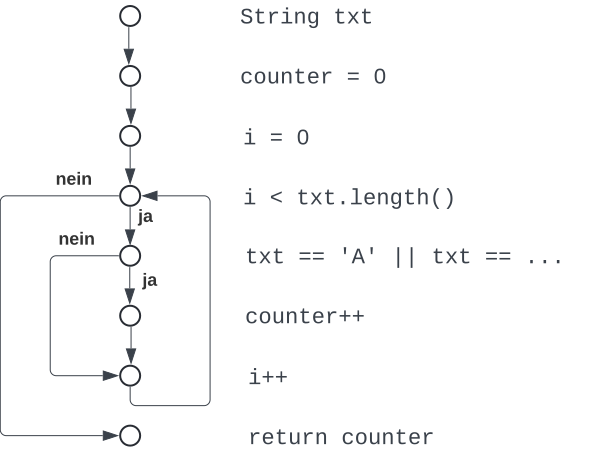
\includegraphics[scale=0.4]{part four/Werkzeuggestützte Analyse/img/kontrollflussgraph}
    \caption{Kontrollflussgraph für \textit{countVowels()}. (Quelle: in Anlehnung an \cite[Abb. 4.1, 32]{Wed09c})}
    \label{fig:kontrollflussgraph}
\end{figure}

\section{Datenflussanomalieanalyse und abstrakte Interpretation}
Es gibt auch Werkzeuge, die unabhängig von Mustern Fehlersituationen anhand der Analyse des Quelltextes erkennen können.\\
Hierzu gibt es zwei Verfahren, die \textbf{Datenflussanomalieanalyse} und die \textbf{abstrakte Interpretation}: Bei beiden Verfahren wird der Zugriff auf Variablen durch mögliche Programmabläufe untersucht (vgl.~\cite[33]{Wed09c}).


\subsection{Datenflussanomalieanalyse}
Die Abfolgen der \textbf{Zugriffe auf Variablen} in den verschiedenen Pfaden eines Kontrollflussgraphen werden bei der \textbf{Datenflussanomalieanalyse} analysiert.\\

\noindent
Zugriffe auf eine Variable werden dazu durch drei Attribute beschrieben (s. Tabelle~\ref{tab:dfaa}):


\begin{table}[]
    \centering
    \setlength{\tabcolsep}{0.5em}
    \def\arraystretch{1.5}
    \begin{tabular}{|c|l|l|}
        \hline
        \textbf{Kürzel} & \textbf{Bedeutung} & \textbf{Beispiel}                                            \\ \hline
        \textbf{d}                                                    & Definition                                                      & \code{x = 5}                                                          \\ \hline
        \textbf{r}                                                    & Referenzierung                                                  & \begin{tabular}[c]{@{}l@{}}\code{y = x + 1}\\ \code{if (x < 4)}\end{tabular} \\ \hline
        \textbf{u}                                                    & Undefinition                                                    & \code{int x;} oder Zerstörung                                         \\ \hline
    \end{tabular}
    \caption{Kürzel in der Datenflussanomalieanalyse und ihre Bedeutung.
    Im Beispiel $y=x+1$ wird $y$ \textit{definiert}, $x$ \textit{referenziert}. (Quelle: \cite[33]{Wed09c})}
    \label{tab:dfaa}
\end{table}

\noindent
Die Abfolge von Attributen in einem Pfad wird als \textbf{Zugriffssequenz} bezeichnet.

\subsubsection*{Beispiel}

Sei folgendes Beispiel in Java gegeben:

\begin{minted}{java}
    class Pair {
        private int min;
        private int max;

        public void minMax() {
            int hilf;
            if (min > max) {
                max = hilf;
                max = min;
                hilf = min;
            }
        }
    }
\end{minted}

\noindent
\code{minMax()} soll überprüfen, ob \code{min} kleiner als \code{max} ist; ansonsten wird der Inhalt beider Variablen vertauschen - was aber im Code nicht umgesetzt ist: Also liegt ein Defekt vor, wie im Folgenden durch die Datenflussanomalieanalyse überprüft werden kann.\\

\noindent
Der Kontrollflussgraph zu \code{minMax} ist in Abbildung~\ref{fig:minmax} gezeigt.

\begin{figure}
    \centering
    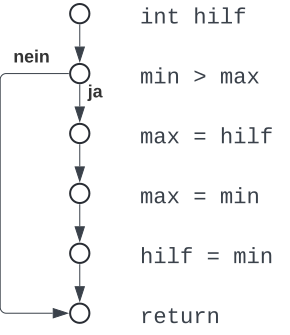
\includegraphics[scale=0.4]{part four/Werkzeuggestützte Analyse/img/minmax}
    \caption{Kontrollflussgraph für \textit{minMax()}. (Quelle: eigene)}
    \label{fig:minmax}
\end{figure}

\noindent
Für die \textit{zwei} möglichen Pfade (\code{min > max} / \code{min <= max}) sind die Zugriffssequenzen der 3 Variablen \code{min}, \code{max} und \code{hilf} in Tabelle~\ref{tab:minmax} aufgelistet.

\begin{table}[]
    \centering
    \setlength{\tabcolsep}{0.5em}
    \def\arraystretch{1.5}
    \begin{tabular}{|c|c|c|}
        \hline
         & \textbf{min > max} & \textbf{min <= max}\\
        \hline
        \code{hilf}                                           & \textbf{urdu}                                          & \textbf{uu}                  \\ \hline
        \code{max}                                            & \textbf{rdd}                                           & \textbf{r}                   \\ \hline
        \code{min}                                            & \textbf{rrr}                                           & \textbf{r}                   \\ \hline
    \end{tabular}
    \caption{Zugriffssequenzen der Variablen für zwei mögliche Pfade in \textit{minMax()}.}
    \label{tab:minmax}
\end{table}

\subsubsection*{3 mögliche Anomalien}
Es gibt bei der Datenflussanomalieanalyse \textbf{3 mögliche Anomalien}, die allesamt in Tabelle~\ref{tab:minmax} auftauchen:

\begin{itemize}
    \item \textbf{ur-Anomalie}: Zugriff auf eine Variable, bevor sie initialisiert wurde.\\
    Der Compiler von Java erkennt diesen Defekt.
    \item \textbf{du-Anomalie}: Definition einer Variable und anschließende Undefinition, ohne, dass sie davor lesend / schreibend verwendet wurde
    \item \textbf{dd-Anomalie}: Mehrmalige Definition einer Variable, ohne, dass zwischendurch lesend auf sie zugegriffen wird.
\end{itemize}

\subsubsection*{Anomalie ungleich Defekt}
\textit{Wedemann} stellt fest, dass die \textbf{ur-Anomalie} einen eindeutigen Defekt darstellt, während das bei der \textbf{dd-} bzw. \textbf{du-Anomalie} nicht so ist: Solche Anomalien können u.a. bei Schleifen auftreten (vgl.~\cite[35]{Wed09c}).

\subsubsection*{Schleifen}
Bei Code mit Schleifen ist die Anzahl der möglichen Pfade für eine vollständige Analyse meistens zu groß: Es reicht aber aus, den abweisenden Fall sowie zwei Durchläufe zu analysieren, da bei den Alternativen prinzipiell keine Anomalien hinzukommen können (vgl.~\cite[35]{Wed09c}).

\subsubsection*{Vorgehen}
Das Vorgehen zur Nutzung solcher Werkzeuge entspricht dem Vorgehen bei den bisher beschriebenen werkzeuggestützten Analyse (s. Abschnitt~\ref{sec:programmierrichtlinien}).
Eine sorgfältige Einweisung der Mitarbeiter ist wichtig.

\subsubsection*{Pro und Contra}
\textbf{ur-Anomalien} werden von vielen Compilern entdeckt.
Zur Entdeckung von \textbf{dd-} bzw. \textbf{du-Anomalien} gibt es nicht viele Werkzeuge\footnote{
für Java gibt es beispielsweise das bereits erwähnte \textit{PMD}, s. Abschnitt~\ref{sec:typische-defekte}
}.
Viele Werkzeuge beschränken sich außerdem auf die Analyse von lokalen Variablen und analysieren keine Instanzvariablen, weshalb der Einsatz der Datenflussanomalieanalyse in den meisten Bereichen nur für qualifizierte Entwickler mit einigen Einschränkungen möglich ist (vgl.~\cite[36]{Wed09c}).
Trotz alledem erlaubt die Datenflussanomalianalyse das Auffinden insb. von Defekten in Zusammenhang mit Schleifen, die sonst nur schwer zu entdecken gewesen wären.

\subsection{Abstrakte Interpretation}\label{subsec:abstrakte-interpretation}
Ähnlich wie bei der \textbf{Datenflussanomalieanalyse} wird bei der \textbf{abstrakten Interpretation} bzw. \textbf{abstrakten Semantik} die Nutzung von Variablen in allen Kontrollflüssen analysiert.\\
Es werden hierbei aber keine Kontrollflüsse \textit{konstruiert}, sondern es kommen aufwändige mathematische Verfahren zum Einsatz.

\subsubsection*{Analyse zugewiesener Werte}
Bei der \textbf{abstrakten Interpretation} wird nicht nur die Art der Nutzung von Variablen, sondern auch der Wert, der ihnen zugewiesen wird, analysiert.\\
\textit{Wedemann} gibt hierzu folgendes Beispiel an (vgl.~\cite[36]{Wed09c}):

\begin{minted}{java}
    public void f(int x) {
        if (x < 10) {
            for (int i = 0; i < x; i++) {
                if (i > 10) {
                    // nicht erreichbar
                }
            }
        }
    }
\end{minted}

\noindent
Zeile 5 ist nicht erreichbar:

\begin{enumerate}
    \item nach Zeile 2 is \code{x <= 9}
    \item nach jedem Schleifendurchlauf wird \code{i} um eins erhöht, bis \code{i == x} als Abbruchbedingung erfüllt ist.
    \item[] Da \code{x <= 9} als Voraussetzung gilt, kann also \code{i > 10} niemals erfüllt werden.
\end{enumerate}

\noindent
Analog wird bei der \textbf{abstrakten Interpretation} bspw. auf
\begin{itemize}
    \item die Überschreitung von Array-Grenzen
    \item Overflow bei skalaren Operationen
    \item Division durch 0
    \item Nutzung durch ungültige Zeiger (C / C++)
\end{itemize}
\noindent
geprüft.

\subsubsection*{Beweis der Abwesenheit von Laufzeitfehlern}
Werkzeuge sind auf diese Art und Weise also in der Lage für Quelltext anzugeben, wo prinzipiell keine Laufzeitfehler auftauchen, und wo sie sicher auftauchen werden.\\
Aus diesem Grund ist der Einsatz von solchen Werkzeugen bspw. im Automotive-Bereich vorgeschrieben (vgl.~\cite[36]{Wed09c}).\\
\textit{Wedemann} verweist ebenda auf \textit{Polyspace}\footnote{
\url{https://de.mathworks.com/products/polyspace.html}, abgerufen 24.05.2024
} als verbreitetes Werkzeug zur Analyse von C, C++ und Ada, merkt aber an, dass die Handhabung kompliziert ist und ein spezielles Training benötigt.

\section{Code-Metriken}
Eine andere Herangehensweise für die werkzeuggestützte Analyse stellt die Ermittlung von \textbf{Code-Metriken} dar.\\
Hierbei werden \textbf{Kennzahlen} bestimmt, anhand derer sich die \textbf{Wartbarkeit} von Source-Code beurteilen lässt.\\
Code-Metriken stehen in \textit{engem Zusammenhang} mit \textbf{Prinzipien guten Entwurfs} (s. Abschnitt~\ref{sec:prinzipien-guten-entwurfs}).\\
Im Folgenden werden die laut \textit{Wedemann} wichtigsten Code-Metriken zur Analyse objektorientierter Software vorgestellt (s. Abbildung~\ref{fig:metriken}).

\begin{figure}
    \centering
    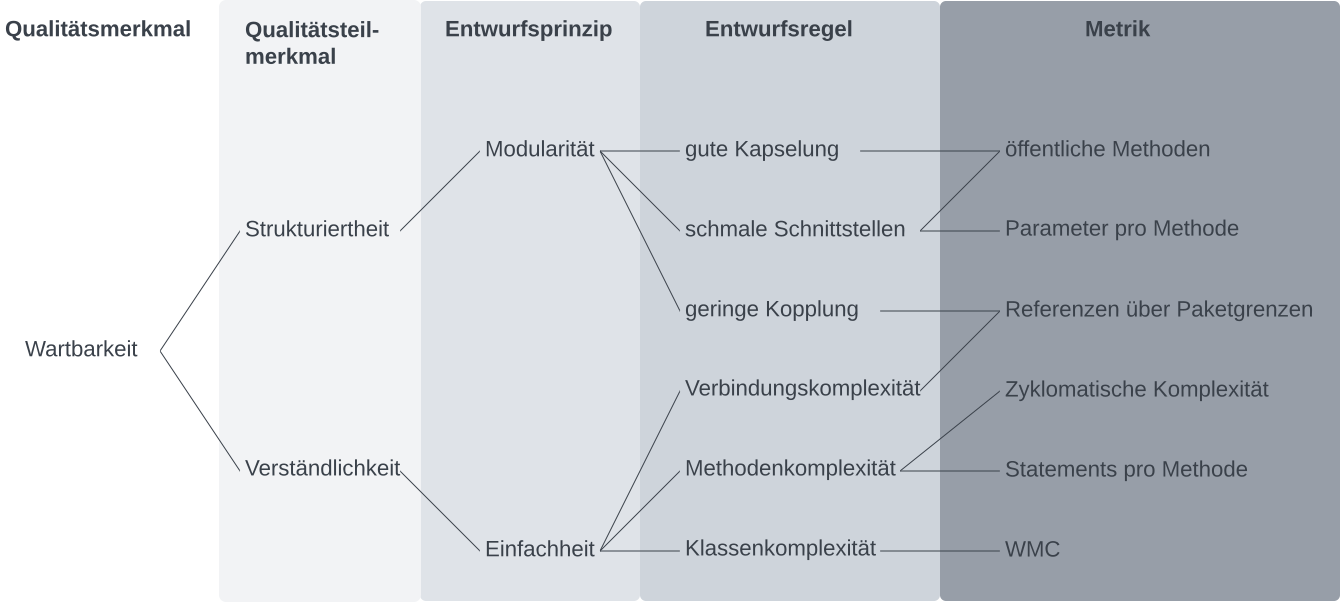
\includegraphics[scale=0.35]{part four/Werkzeuggestützte Analyse/img/metriken}
    \caption{Typische Metriken zur Bestimmung des \textbf{Qualitätsmerkmals} \textit{Wartbarkeit} und ihr Zusammenhang mit den Qualitätsteilmerkmalen. \textbf{WMC} steht für  \textit{Weighted Mean Complexity} (s. ``Komplexität``). (Quelle: in Anlehnung an \cite[Abb. 4.3, 37]{Wed09c})}
    \label{fig:metriken}
\end{figure}

\begin{tcolorbox}[colback=white]
    \textbf{Wartbarkeit} von Code ist immer auch abhängig von den Qualitätsteilmerkmalen \textbf{Strukturiertheit} und \textbf{Verständlichkeit}, die sich mit Metriken messen lassen.\\
\end{tcolorbox}
\vspace{2mm}

\noindent
Folgende Qualitätsteilmerkmale werden erfüllt, wenn der Entwurf bestimmte Regeln bzw. Prinzipien befolgt, die sich dann in der Implementierung widerspiegeln:

\begin{itemize}
    \item gut strukturierter Code ist leichter zu ändern
    \item einfach zu verstehender Code lässt sich leichter ändern
\end{itemize}

\begin{tcolorbox}
    Ob die Qualitätsforderung \textbf{Wartbarkeit} erreicht ist, kann auch durch Code-Metriken überprüft werden, die versuchen, Prinzipien wie \textbf{Modularität} und Regeln wie \textbf{geringe Kopplung} in Zahlen zu fassen (vgl.~\cite[38]{Wed09c}).
\end{tcolorbox}
\vspace{2mm}

\subsection*{Modularität}
Wenn Quellcode \textbf{modular} ist, ist er auch \textbf{gut strukturiert}.\\
Zur Messing von \textbf{Modularität} werden Metriken zu 3 \textbf{Entwurfsregeln} betrachtet:

\begin{enumerate}
    \item \textbf{gute Kapselung} entsteht durch \textit{wenige} \textbf{öffentliche Methoden}
    \item \textbf{schmale Schnittstellen} bewirkt eine \textbf{niedrige Kopplung}: Dies wird insgesamt erreicht durch \textit{wenig öffentliche Methoden} mit einer \textit{geringen Anzahl von Parametern}\footnote{
    s. auch \textit{Data Coupling}, Abschnitt~\ref{subsec:lose-kopplung}
    }
    \item \textbf{geringe Kopplung von Paketen} wird erreicht, indem wenige Referenzen über Paketgrenzen hinausgehen.
\end{enumerate}


\subsection*{Zyklomatische Zahl}
Zur Abschätzung der \textbf{Komplexität einer Methode} wird häufig die \textbf{zyklomatische Zahl} (auch: \textit{McCabe-Metrik}\footnote{
s. \url{https://de.wikipedia.org/wiki/McCabe-Metrik}, abgerufen 25.05.2024
}) verwendet.\\
Sie gibt die Anzahl unabhängiger Zyklen an, also die Anzahl der Verzweigungen in einer Methode $+1$.\\
Formal lässt sich die \textbf{zyklomatische Zahl} aus dem \textbf{Kontrollflussgraphen} bestimmen: Mit $n$ als Anzahl der Knoten und $e$ als Anzahl der Kanten berechnet sich die zyklomatische Zahl zu $Z = e - n + 2$.\\
Ist eine zyklomatische Zahl hoch, wird von einer hohen Komplexität ausgegangen.\\
Als Beispiel sei nochmals der Kontrollflussgraph zu der Methode \code{countVowels()}\footnote{
    s. Abschnitt~\ref{sec:hilfsmittel-kontrollflussgraph}
} gegeben (s. Abbildung~\ref{fig:zyklomatischezahl}):  Mit $n = 8$ und $e = 9$ berechnet sich die zyklomatische Zahl zu $e - n + 2 = 9 - 8 + 2 = 3$


\begin{figure}
    \centering
    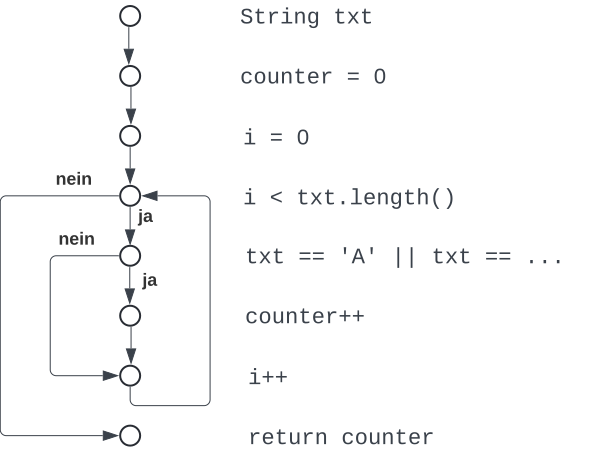
\includegraphics[scale=0.4]{part four/Werkzeuggestützte Analyse/img/kontrollflussgraph}
    \caption{Kontrollflussgraph für \textit{countVowels()}, für den sich eine zyklomatische Zahl von $Z=3$ ergibt. (Quelle: in Anlehnung an \cite[Abb. 4.1, 32]{Wed09c})}
    \label{fig:zyklomatischezahl}
\end{figure}

\noindent
\textit{Wedemann} merkt an, dass die zyklomatische Zahl von zwei \textit{verschachtelten} Schleifen oder Bedingungen genauso groß sei wie die von zwei aufeinanderfolgenden Schleifen oder Bedingungen, obwohl verschachtelte Konstrukte meist schwerer verständlich sind, und dass eine zyklomatische Zahl von $>10$ von vielen Autoren als problematisch betrachtet wird\footnote{
McCabe verwendet in seinem Paper $10$ als ``a reasonable, but not magical,  upper limit.`` (\cite[314]{McC76})
} (vgl.~\cite[38]{Wed09c}).


\subsection*{Komplexität}
Ein weiteres Maß für die \textbf{Komplexität einer Methode} ist die \textbf{Anzahl der Anweisungen}\footnote{auch: Anzahl der Zeilen. Eine Anweisung kann über mehrere Zeilen gehen.}.
Lange Methoden sind sicherlich schwieriger zu verstehen, weshalb auch hier weniger Anweisungen besser sind.\\
Die \textbf{Komplexität einer Klasse} kann mit Hilfe der \textbf{Weighted Mean Complexity} (\textit{WMC}) gemessen werden, für deren Bestimmung die zyklomatische Zahlen \textit{aller Methoden} zusammengezählt werden - auch hier ist ein geringerer Wert besser.

\subsection*{Vorgehen}
Für den Umgang mit den berechneten Zahlenwerten gibt es zwei Strategien:

\begin{enumerate}
    \item Zu den verschiedenen Metriken sind in der Literatur oder den Werkzeugen typische Grenzen angegeben, innerhalb derer Code als ``gut`` betrachtet werden kann.
    \item Da die in (1) erwähnten Grenzen willkürlich erscheinen können bzw. sich verschiedene Quellen bei der Angabe der Grenzen widersprechen können, werden Projekte oft mit einem Satz von Standardwerten untersucht und dann ggf. an das Projekt angepasst.
\end{enumerate}

\noindent
Werden Metriken in einem bereits fortgeschrittenen Projekt eingesetzt, sollten nur die Klassen und Methoden untersucht werden, die besonders auffällig sind.

\subsection*{Werkzeuge}
Für Java gibt es bspw. \textit{Metrics}\footnote{
\url{https://metrics.dropwizard.io}, abgerufen 25.05.2024
}, für PHP bspw. \textit{PHPMetrics}\footnote{
    \url{https://www.phpmetrics.org}, abgerufen 25.05.2024
}.

\subsection*{Pro und Contra}
Code-Metriken sind ein bewährtes Mittel zur Analyse von Code in Bezug auf \textbf{Wartbarkeit}.\\
Wenn Metriken parallel zur laufenden Entwicklung eingesetzt werden, können viele Schwachstellen vermieden werden - sie sind allerdings auch geeignet, um in fremden Code Schwachstellen zu entdecken, wodurch sie ein wertvolles Werkzeug für Projektleiter, QS-Verantwortliche und auch Kunden sind (vgl.~\cite[39]{Wed09c}).\\
In der Praxis kann es sich als schwierig erweisen, geeignete Metriken auszuwählen und die ermittelten Daten korrekt zu interpretieren: Hier werden fehlerhafte Ergebnisse dann durch ungeeignete oder falsch interpretierte Metriken verursacht, was zu Ablehnung der Werkzeuge führen kann.\\
Es ist also ratsam, sich in die einzusetzenden Metriken einzuarbeiten und an bekannten Projekten zunächst auszuprobieren.

\section{Zusammenfassung}


\begin{itemize}
    \item Sequenzdiagramme sind \textbf{Verhaltensdiagramme}
    und können im gesamten Entwicklungszyklus zur Modellierung von Interaktionen angewendet werden
    \item Interaktionen bestehen im Wesentlichen aus dem Nachrichtenaustausch zwischen verschiedenen Kommunikationspartnern
    \item in den meisten Fällen wird die Kommunikation von Objekten von Klassen modelliert, aber es können auch Teilnehmer auf anderen Ebenen modelliert werden
    \item gewöhnlich gibt ein Sequenzdiagramm einen \textbf{Anwendungsfall} (\textit{Szenario}) wieder
    \item sie dienen nicht dazu, um Zustandsänderungen darzustellen (hierfür werden Zustandsdiagramme verwendet)
    \item Sequenzdiagramme sind \textit{nicht} gut geeignet für die Darstellung von
    \begin{itemize}
        \item nebenläufigem Verhalten (\textit{asynchrone} Nachrichten, \textit{kombiniertes Fragment})
        \item Schleifen und alternativem Verhalten (\textit{kombinierte Fragmente})
        \item[] $\rightarrow$  für beide Fälle sind \textbf{Aktivitätsdiagramme} besser geeignet
    \end{itemize}
\end{itemize}
\newpage


